\chapter{Roles of literature}

In this chapter I examine how the composed topics and their dynamics over time relate to prevailing theses drawn from contemporary qualitative research on the role of early modern literature, which I already discussed in Chapter 1, \textit{Introduction}. I discuss each claim in more detail, after which I explore whether the claim can be validated with the obtained results.

\section{Literature and ideology}
In the Introduction, I already discussed how literature is seen as a propagator of an ideology and how this is the case for the literature of the pietistic tradition. I also made clear in the previous chapter, that religion is by far the most dominant topic in my corpus. From the fifty topics that were built, eighteen have, more or less, something to do with religion. Regarding the Top10 most dominant topics, six of them are on religion. In Figure~\ref{fig:religion}, I plotted the evolution of these six topics over time. The y-axis shows the number of songs with a certain topic as their most dominant topic; the x-axis shows the development of a topic's popularity through time. Table~\ref{table:DomTopVARD2extended} already showed that topic 9 was by far the most dominant topic in my corpus. Figure~\ref{fig:religion} makes clear that this topic was mainly popular in the sixteenth century: it even almost disappears after 1650. There is a clear explanation for that, to which I already referred in assigning the subject \textit{religion and old spelling} to this topic. It contains words in a typical fifteenth and sixteenth-century spelling, ages in which no clear difference between the printed letters \enquote{v}, \enquote{w} and \enquote{u} existed, resulting in words such as \enquote{wt}, \enquote{bouen}, \enquote{uan}, \enquote{verheuen}, and \enquote{blijuen}. These words were not normalized by the VARD2-tool. An explanation for this is that the tool was trained on more recent texts (dating from 1637 and 1657), in which words were spelled according to more modern spelling conventions. Variants that were common in earlier centuries, were therefore probably not included in the variant-list. Another reason might be that these interchangeable letters, such as \enquote{v}, \enquote{u}, and \enquote{w}, are mainly a result of poorly transcribed prints. It can be said anyway that this topic 9 is not actually a topic, but merely a cluster of old-fashioned words that were still used between 1550 and 1625, and that these words disappear from the vocabulary of song lyrics when the seventeenth century endures.

\begin{figure}[hbt!]
	\centering
	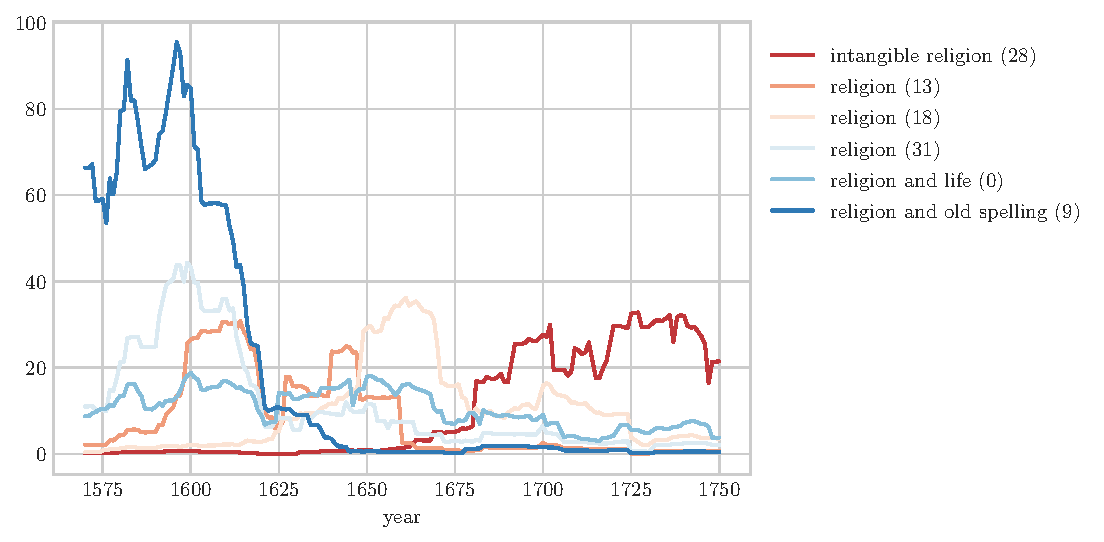
\includegraphics[scale=0.8]{religion}
	\caption{Topics on religion from the Top10}
	\label{fig:religion}
\end{figure}

Dynamics within the other five topics can be easier observed in a graph without topic 9. This plot (see Figure~\ref{fig:religion_min_9}) shows that the topics 13, 18 and 31, to which I was not able to assign a more detailed subscription than \textit{religion}, follow each other roughly. It starts with topic 31, peaking just before 1600, succeeded by topic 13 which culminates in the first half of the seventeenth century. Topic 18 closes the row, peaking in the second half of the seventeenth century. Looking in more detail to the words from which the topics were composed, does not give that much insight, but in the Intertopic Distance Map, made with \texttt{pyLDAvis} (Figure~\ref{fig:pyLDAvisVARD2}), topics 13 and 31 overlap very much in the bottom right quadrant. This overlap can also be observed when looking at their graph lines: both topics peak almost at the same time. Topic 18 is positioned in the upper right quadrant in Figure~\ref{fig:pyLDAvisVARD2}, the same quadrant where topic 28 is located: the topic on \textit{intangible religion} that succeeds topic 18, according to the plot in Figure~\ref{fig:religion_min_9}. There is a clear trend in the graph line of topic 28: until 1650 this topic hardly exists, but afterwards the line shows a quickly increasing slope. Until 1750, where my corpus ends, this topic on \textit{intangible religion} dominates. I already explained in the previous chapter that, in this topic, words prevail that are related to the intangible aspects of the Christian faith.

\begin{figure}[hbt!]
	\centering
	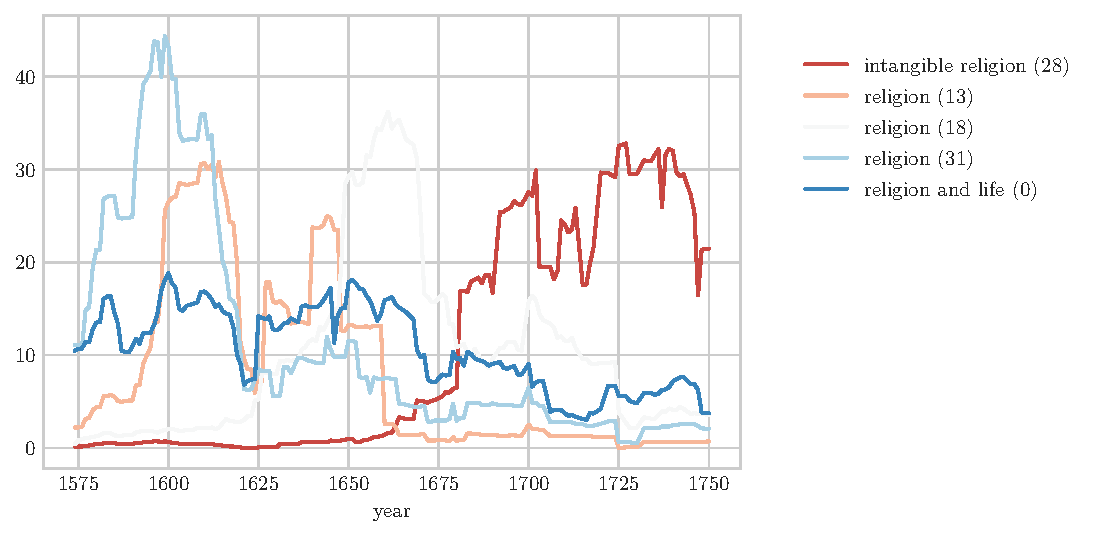
\includegraphics[scale=0.8]{religion_min_9}
	\caption{Topics on religion from the Top10 (except topic 9)}
	\label{fig:religion_min_9}
\end{figure}

\begin{figure}[hbt!]
	\centering
	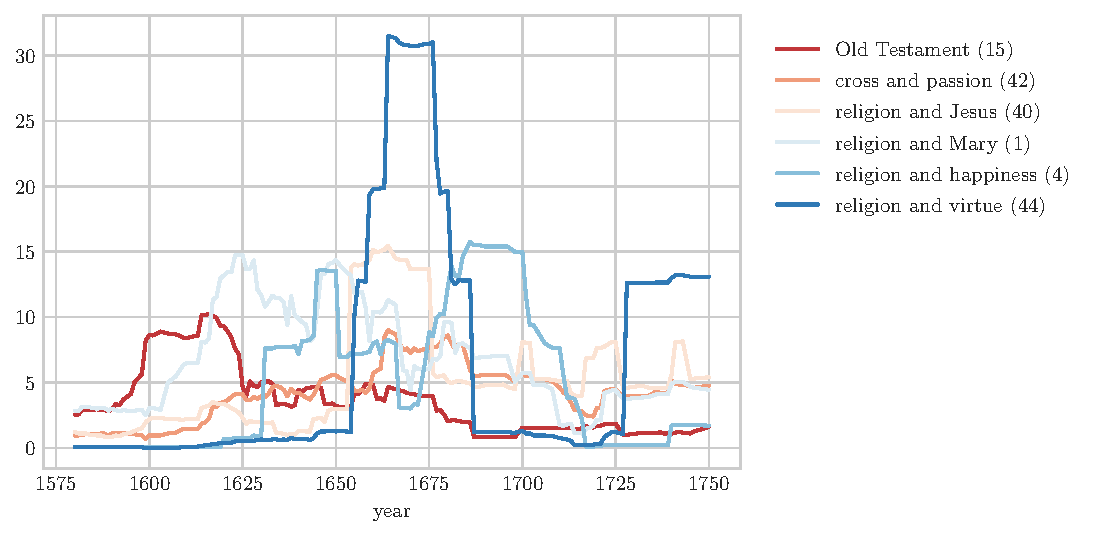
\includegraphics[scale=0.8]{religion2}
	\caption{Topics on religion from the lower parts of the chart}
	\label{fig:religion2}
\end{figure}

Since the sudden increase of this topic coincides with the rise of the pietistic tradition in the Low Countries called the Further Reformation, topic 28 clearly represents one of the two trends Porteman and Smits-Veldt determined in literary texts from this movement. On the one hand, literary texts with a focus on a sanctification on society and all aspects of life, prevailed. On the other hand, texts appeared in which the personal lived experience with God was described and expressed. These latter are brought together in topic 28. Figure~\ref{fig:religion2} shows that the other religious topics, which were located lower in the chart, do not demonstrate a striking curve, except the \enquote{Domtower-ish} shape of topic 44, belonging to \textit{religion and virtue}. Since the sudden rise of this topic is located in the second half of the seventeenth century as well, this seems to fit with the first trend of the literary texts from the Further Reformation that Porteman and Smits-Veldt determined. \autocite[658]{porteman_een_2009} Dominant words in this topic that confirm these thoughts, are \enquote{deughden}, \enquote{bidt}, \enquote{leven}, and \enquote{vroom}. The twofold ideology the advocates of the Further Reformation wanted to propagate according to contemporary research, is cleary represented in the obtained quantitative results.

\section{Literature and poetics}
I expect the relationship between literature and poetics to be most apparent in love topics that can be related to Petrarchism. Francesco Petrarca (1304 - 1374), godfather of this movement, was an Italian poet from the fourteenth century, who became famous all over Europe during the early modern centuries. One of the reasons for this was because he started to write poetry in the Italian vernacular, and based on the classics. This was a great inspiration for Dutch poets in the sixteenth and seventeenth century, who were searching for their own identity, during a war for political and religious independence.\autocite[17]{porteman_een_2009} The other reason for Petrarca's fame in the Netherlands was the popularity of his poetry on love. Distinctive of Petrarca's love sonnets, was the worship of a charming but unreachable woman. As a result of that, love always causes both happiness and pain in his poems. The physical beauty of the beloved is often described, using natural metaphors and mythological references. The lover owns a split personality, and often struggles with suicidal tendencies.\autocite{bork_algemeen_2012} 

Regarding the results obtained in the previous chapter, the second-largest overarching category of topics is love. The two most dominant topics in this category, are two contradictory ones: topic 39 is on \textit{love and sadness}, topic 38 is on \textit{love and happiness}. In Figure~\ref{fig:love} I plotted the two topics through time, which shows an interesting pattern. What immediately stands out, is that the topics only start to occur around 1630. From that point in time, \textit{love and sadness} is the most dominant topic, culminating around 1660, but decreasing quickly afterwards. Around 1710, the line of topic 38 on \textit{love and happiness} suddenly rises, and rapidly becomes the dominant one of the two love topics. This plot suggests that song with negative emotions are replaced by songs with a more light-footed view on love. The question is if that trend is confirmed by other topics on love. Therefore I included more love-topics to the plot, resulting in the graph of Figure~\ref{fig:love_extended}. Prior to topic 39, topic 2 starts the list of topics on love. This topic, on \textit{love and tragedy}, dominates between 1575 and 1630. What follows, is a couple of overlapping peaks, all culminating around 1660, with the topic on \textit{love and sadness} as most dominant one. The smaller peaks belong to \textit{rejection}, \textit{seducing} and \textit{physical love}.

\begin{figure}[hbt!]
	\centering
	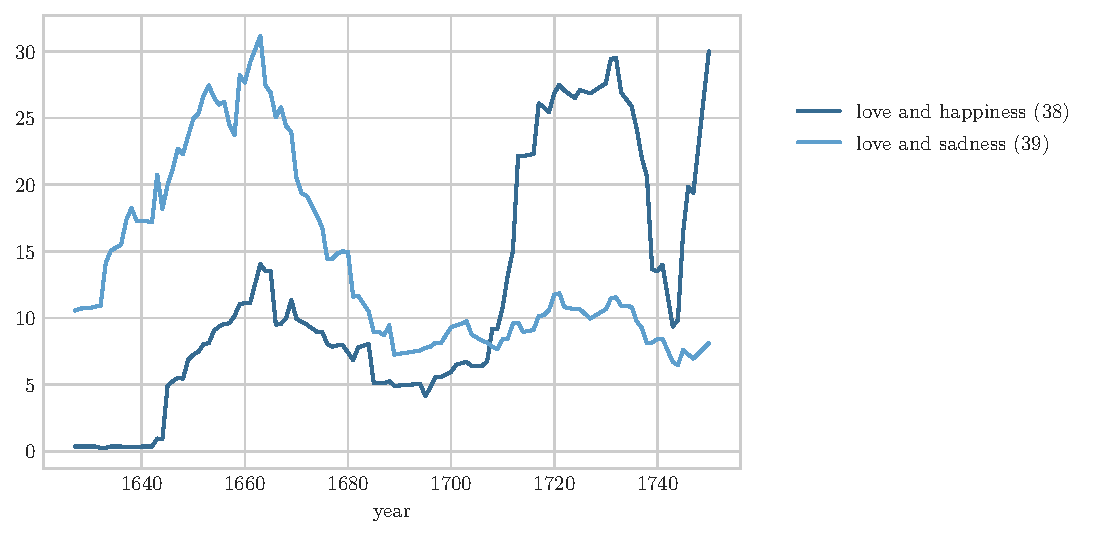
\includegraphics[scale=0.8]{love}
	\caption{\textit{love and happiness} versus \textit{love and sadness}}
	\label{fig:love}
\end{figure}

All these topics, dominating the sixteenth and seventeenth century love topics, can be related to the heydays of the Petrarchism. The most famous imitators of Petrarca in the Netherlands were poets Jan van der Noot (1539 - 1595) and Pieter Corneliszoon Hooft (1581 - 1647).\autocite[46, 206]{porteman_een_2009} In most of the poems Hooft wrote, he adhered to the international conventions of amorous lyric, in which Petrarca's poetry strongly resonated. The case of Hooft demonstrates that not only poems, but songs as well, were written according to Petrarcian standards. Hooft's songs ended up in song books, accompanied with melodies, and reached a large audience.\autocite[46, 206]{porteman_een_2009} Porteman and Smits-Veldt argue that, from 1607, song poets referred in their melody assigning to songs from Hooft's play \textit{Granida} (1605).\autocite[206]{porteman_een_2009} These are the trends I see reflected in Figure~\ref{fig:love_extended}, where topics, who all in their own way relate to Petrarcian love poetry, dominate between 1575 and 1650.

\begin{figure}[hbt!]
	\centering
	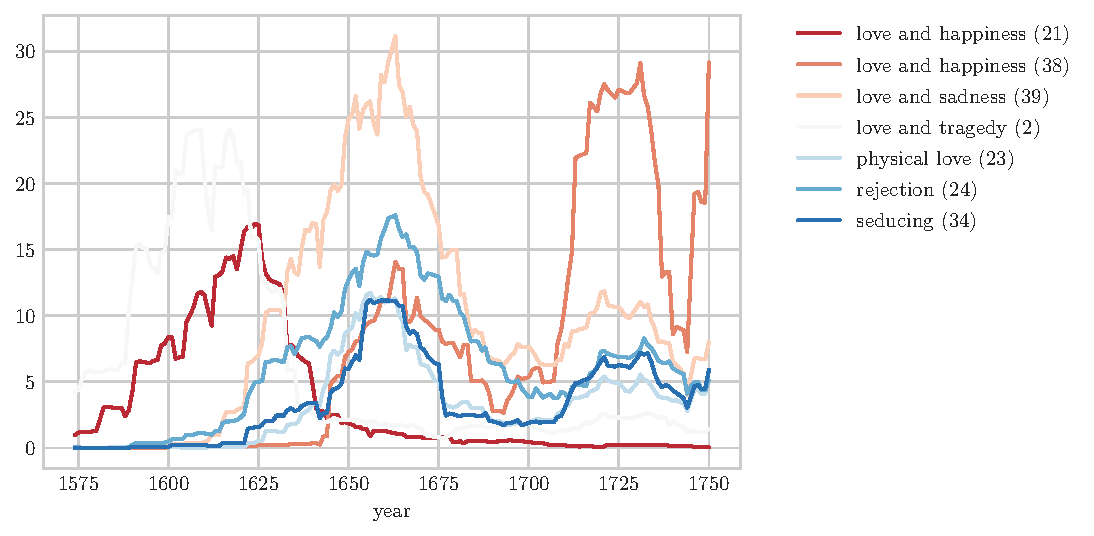
\includegraphics[scale=0.8]{love_extended}
	\caption{Love topics}
	\label{fig:love_extended}
\end{figure}

Other topics which can be related to the humanistic tradition, are \textit{bucolic songs} (47), \textit{myth and beauty} (14) and \textit{nature} (37), which I plotted in Figure~\ref{fig:bucolic}. With \enquote{bucolic}, I refer to the \enquote{pastorale} or \enquote{sheperd's song}, a popular genre in the seventeenth century. The bucolic song originates from the classics, when poets such as the Greek Theocritus and the Roman Virgil were famous bucolic poets. The use of mythological figures, such as \enquote{venus} and \enquote{phoebus} from topic 14, indicates the imitation of classical genres and topics.

\begin{figure}[hbt!]
	\centering
	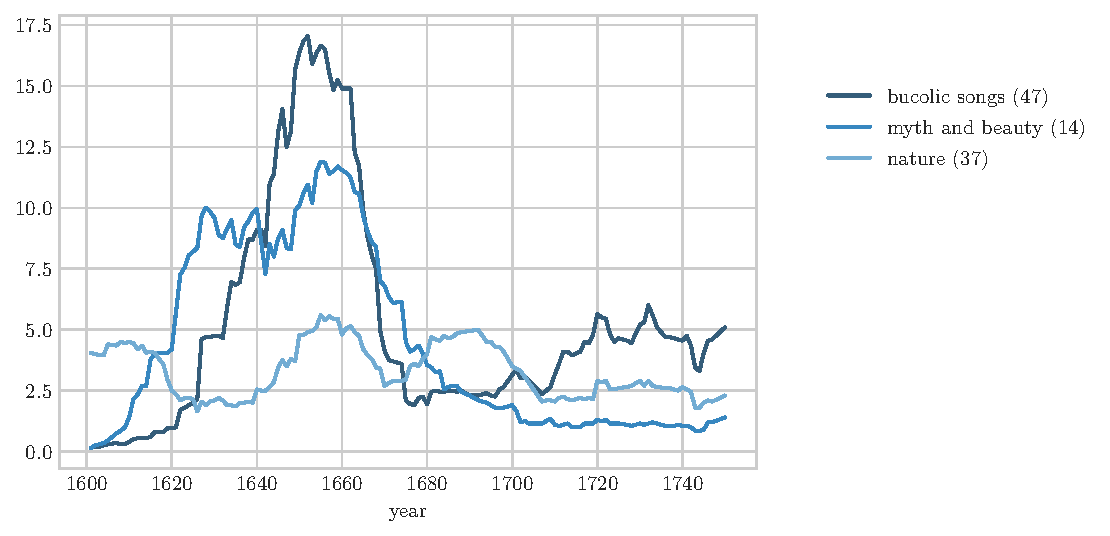
\includegraphics[scale=0.8]{bucolic}
	\caption{Renaissance topics}
	\label{fig:bucolic}
\end{figure}

As from 1660, I see a clear decline of these topics. It is important to realize, though, that the total distribution of songs in my corpus declines as well as the seventeenth century ends (but inclines again at the beginning of the eighteenth century). Still, an evident pattern can be observed in the love topic distribution in the eighteenth century. Topics on \textit{love and sadness}, \textit{love and tragedy} and \textit{rejection} are overruled by a topic on \textit{love and happiness}. According to Figure~\ref{fig:love_extended}, the Petrarcian tradition seems to move to the background, making room for a less dramatic, and more light-footed interpretation of love.

\section{Literature and politics}
Regarding the relation between literature and politics, I already mentioned the claim from contemporary research that, during political crises, literature with such crises as subject is written and read more often. If that is correct, I should see an increase of topics related to country, war and enemy, during times in which the Dutch Republic was in a precarious political situation. Although war was more of a rule than an exception in the history of the Dutch Republic, there are for sure some moments to indicate in which the crisis was peaking. First and foremost there is the Eighty Years' War, lasting from 1568 until 1648, in which the Dutch struggled for independence from the Spanish king. Although the war was interrupted for the Twelve Year's Truce, which was set from 1609 until 1621, this did not lead to a quite and carefree period in the Dutch Republic: two factions emerged as result of a theological disagreement between two professors in theology from the University of Leiden about the predestination. The debate was not limited to the religious discourse, but grew into a national conflict, concerning the question how and by whom the correct dogmas of the Reformed Church (\enquote{Gereformeerde Kerk}) should be decided.\autocite[40]{prak_gouden_2012} The conflict culminated in 1619 in the death sentence of Johan van Oldebarnevelt, the land's advocate of the Republic, simultaneously with the Synod of Dort in which the controversy around the remonstrants and counter-remonstrants was settled by sentencing counter-remonstrantism to heresy. As a result, prince Maurits managed to end the intern agitation before the Truce itself ended.\autocite[47]{prak_gouden_2012} In the end, the dispute ensured an uninterrupted uproar in the Republic for eighty years, since the Revolt continued after the Twelve Year's Truce ended in 1621. After an up and down wavy continuation of the battle, without a substantial difference in power, the Peace of Münster was finally signed by the Dutch Republic and the Spanish Crown in the winter of 1648, indicating the end of the Revolt.\autocite[53]{prak_gouden_2012} Summarized, if there is one period in which songs with nation and war as topic should be excelling, it has to be during the Dutch Revolt.

The results from the last paragraph of Chapter 7 already showed that, after adding reprints to my corpus, the topic on \textit{nation and country} is positioned at the bottom of the Top10 dominant topics. Related topics seem to be topic 7 on \textit{God and enemy} and topic 49 on \textit{God and country}, and therefore I plotted these three topics together in Figure~\ref{fig:nation}. It turns out that \textit{nation and country} starts to appear as most dominant topic of a song around 1580. Striking is the fact that the line does not start close to zero, but close to ten: the songs seem to appear almost out of nothing. In the next forty years, the number of songs per year with this topic as their dominant one, only rises. This sudden increase in popularity clearly indicates that songs with this topic were written, read and sung much more often during that time. Dominant words show that this topic is indeed on the Revolt, which is mainly illustrated by words as \enquote{prins}, \enquote{land}, \enquote{graaf}, \enquote{spaensche} and \enquote{paus}. This confirms the hypothesis that there should be an increase of topics related to country, war, and enemy, during the Eighty Years' War. In the previous chapter I already suggested that the Geusen songbooks were probably largely responsible for the sudden popularity of this topic. The line of topic 32 in Figure~\ref{fig:nation} confirms that expectation: it appears around the same time as the oldest known edition of \textit{Een nieu geuse lieden boexcken} dates from, which is the year 1577 or 1578.\autocite[75]{porteman_een_2009} Around 1640, the graph line of topic 32 shows a drastic fall, which can be explained with the end of the Dutch Revolt in 1648.

\begin{figure}[hbt!]
	\centering
	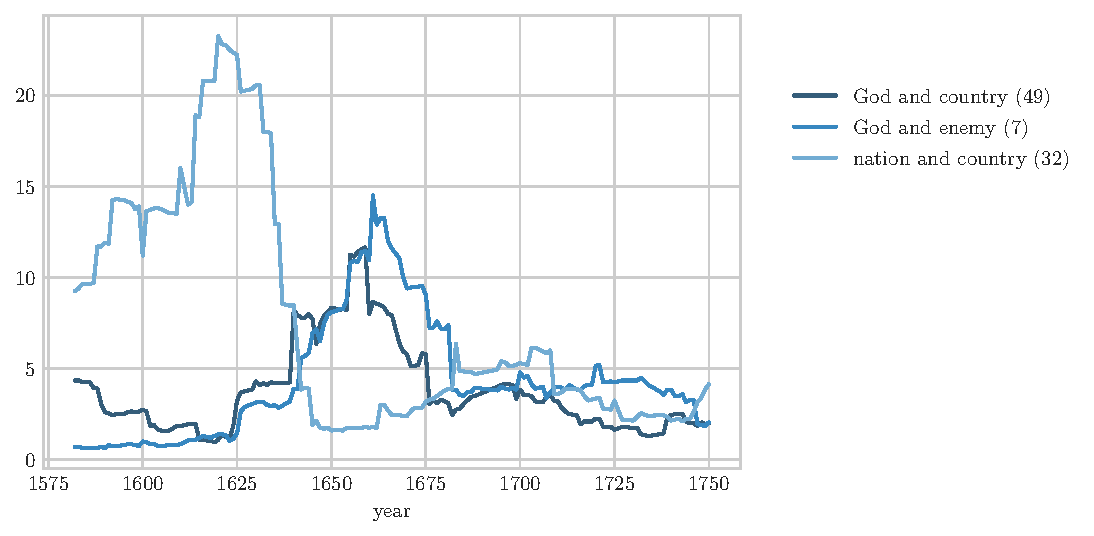
\includegraphics[scale=0.8]{nation}
	\caption{Nation, country and politic topics}
	\label{fig:nation}
\end{figure}

Remarkable is that, at the same time, two other relatable topics are rising, namely the one on \textit{God and country} (49) and \textit{God and enemy} (7). However, this does not come as much as a surprise, if you realize that the peace in the Dutch Republic only lasted until Stadtholder William II did a failed attempt to take over the city Amsterdam and therefore increase his power in 1650.\autocite[55]{prak_gouden_2012} He died a couple of months later, leaving his highly pregnant wife behind. It was the start of the First Stadtholderless period, which lasted until 1672. Again, the Dutch Republic was in turbulent waters. Although they were much more important than many a monarchy in the second half of the seventeenth century, the search for a new balance of power in Europe was accompanied by a long series of wars. Between 1652 and 1674, the Republic fought three wars with England.\autocite[57]{prak_gouden_2012} That could be an explanation for the topics on country and enemy that are still prevalent, after the end of the Revolt.

However, there are some differences between topic 32 on the one hand, and the topics 7 and 49 on the other hand. An important contrast is the major absence of religious words in topic 32. The word \enquote{god} is part of this topic, but it is the only word from the religious domain, and, moreover, it is less prevalent than words such as \enquote{prins}, \enquote{land}, \enquote{stad} and \enquote{vijand}. The topics 7 and 49, however, contain much more overlap with other religious topics, with the presence of words such as \enquote{god}, \enquote{boze}, \enquote{gods}, \enquote{handen} in topic 7, and \enquote{god}, \enquote{zijnen}, \enquote{naam}, \enquote{heren} and \enquote{hemel} in topic 49. I therefore suspect that these songs are religious songs with a strong focus on the aspect of war, peace, enemy, and the people. The song with the highest contribution of topic 49, turns out to be a psalm in the translation of Petrus Datheen (\texttt{id} =  7998), the song with the highest contribution of topic 7 is from the songbook \textit{Stichtelijcke Gesangen, behelsende: Bybelsche In-vallen. Geestelijcke Bedenckingen. Eerlijcke Vermaeckingen.} from 1661 (\texttt{id} = 155823). It is therefore also possible that the rise of these two topics has something to do with the earlier mentioned rise of reformed songbooks after 1650.

\section{Literature and diversity}
The last claim on the role of literature in early modern times I will test, is the one on diversity of both the people that were involved with literature, as well as the topics in literature. I already cited Veldhorst, who made clear that poor and rich, young and old were engaged with songs during the seventeenth century.\autocite[217]{veldhorst_pharmacy_2008} Furthermore, several studies have shown that songbooks printed especially for young readers started to appear at the beginning of the seventeenth century.\footnote{See for example \autocites{stronks_dees_2014}{grootes_het_1987}.} Their number only increased as the years passed. In the introduction of a twentieth century edition of G.A. Bredero's \textit{Groot lied-boeck}, F.H. Matter designates the publication of \textit{Den nieuwen Lust-hof} in 1602 as the beginning of a new era, in which more and more songbooks appear that are especially intended for the youth, as appears from their title or preliminary work.\autocite[18]{bredero_g._1975} A major part of the songs were on love, but not all of them. Matter asks himself why poets and printers were keen to gain the favor of the youth by producing songbooks especially for them. He does not believe that their one and only reason was the fact that youth is continuously in love and therefore yearns for love songs. Other possible explanations Matter mentions, are that youth represents a potential market since they were rather prosperous, that they are not yet seized by household worries, and that youth can be related to modern, anti-traditional and sensitive to new movements in art and literature.\autocite[19]{bredero_g._1975}

Another group that became more and more involved in literature, are women. Although male authors dominate the literary history, we know from several studies that female authors and readers were not absent during the early modern centuries. The extensive study \textit{Met en zonder lauwerkrans. Schrijvende vrouwen uit de vroegmoderne tijd 1550-1850: van Anna Bijns tot Elise van Calcar} on writing women in the early modern time shows that women were active in both the profane and religious domain, and in very different genres.\autocite{schenkeveld-van_der_dussen_met_1997} The sisters Anna and Tesselschade Roemers Visscher, Katharina Lescailje and Titia Brongersma are the most famous examples of female poets, but Schenkeveld-van der Dussen et al. determine more than seventy female writers from the seventeenth century alone. Women wrote poetry on all sorts of worldly subjects, mostly published in anthologies. Porteman and Smits-Veldt notice that, in contrast to male poets who started to publish collection bundles from the second half of the seventeenth century, this did not happen for the literary works by women.

Regarding female poets who wrote religious poetry, they put themselves completely at the service of the purpose of their texts: spiritual foundation and consolation.\autocite[840]{porteman_een_2009} Many of them were pastor's wives, and their work was in line with the tradition of the Further Reformation. From about 1670, collection bundles from female poets began to be published as well. These bundles were for the most part filled with poetry on religious subjects, and sometimes alternated with poets on worldly subjects. Authors from such mixed bundles saw their writership as subservient to the religious community they belonged to. If they discussed worldly subjects in their poetry, this happened still in a religious perspective. In some cases, the intended public of female writers were women as well. The addressates of sixteenth-century poet Vrou Gerrits' bundle are her sisters in Christ, and for Cornelia Teellinck's work, a female readership is assumed as well.\autocite[51]{schenkeveld-van_der_dussen_met_1997} Geertruida Sluiter states explicitly that she is writing to clearly formulate her faith and help fellow females with that. However, we can not assume that women were only writing for women, since there are as much examples that prove the opposite, for example the works of the eighteenth-century poet Geertruyd Gordon.\autocite[840]{porteman_een_2009} 

With the methods used in this thesis and the results obtained with it, it is hard to check whether the above claims are confirmed by quantitative research. I can see that certain love topics become more and more prevalent indeed, but topics do not give me insight in the writer of a lyric or the intended public of a song. It is possible that there are changes in the gender of characters that are subject of a lyric, but the use of a stop list ensures that personal pronouns which might suggest something on this, are excluded from the composed topics. To test the above claims, other quantitative methods should be used, for example an analysis of the preliminary works of songbooks to get insight in the intended public of a literary work.

My methods are more useful to say something about the growing diversity of topics in my corpus over time. The turnover, which I discussed previously in Chapter 3 and Chapter 6, can show me if the same topics stay the most popular over a longer period of time, or if the composition of the upper part of the ranking constantly, or during a certain time period, shifts. To compute the annual turnover of topics, I followed the steps I formulated earlier in Chapter 6. From the DataFrame I created in Chapter 7, I extracted the most dominant topic for each song. Afterwards I grouped these topics by year, and counted the number of appearances for each topic in every year. In this way, I could create an annual popularity index, containing all song topics, ranked according to their frequency of appearance in descending order. I used the following block of code:

\begin{lstlisting}
import numpy as np
import pandas as pd

top3topicsong = pd.read_csv("top3topics_allsongs.csv", sep="\t", index_col=0)
groups = top3topicsong.groupby("year")

year2index = {year: i for i, year in enumerate(sorted(top3topicsong.year.unique()))}
X = np.zeros((top3topicsong.year.unique().size, 50))
counts = groups["top1"].value_counts()
for (year, topic), count in counts.iteritems():
topic = int(topic.replace("topic ", ""))
X[year2index[year], topic] += count

turnovertop1 = np.array([x[::-1] for x in X.argsort(1)])
\end{lstlisting}

\noindent The result is a \texttt{numpy} matrix in which each array corresponds with a year, and consists a list of topics, ranked from the most dominant to the least dominant. Note that the length of the matrix is 196: the years are numbered from 0 to 195. This means that five years, from which no songs are present in my corpus, are excluded from the matrix. It concerns the years 1555, 1606, 1691, 1726, and 1729. For each position in the ranked lists, I count the number of \enquote{shifts} in the ranking that have taken place between two consecutive years. This \enquote{number of shifts} is called the turnover. Computing the turnover for all time steps in our collections yields a turnover series.

However, calculating the turnover of this ranking would not make sense, since all fifty topics appear in each ranking every year. The number of shifts would therefore always be zero, resulting in a flat graph line. Therefore I use a cutoff, to only include the upper part of the ranking in the calculation of the annual turnover. I use the following code for that (after I converted the \texttt{numpy} matrix to a \texttt{pandas} DataFrame):

\begin{lstlisting}
df_turnoverseries = pd.DataFrame(turnovertop1)
cutoff5 = df_turnoverseries[[0, 1, 2, 3, 4]].copy()
cutoff10 = df_turnoverseries[[0, 1, 2, 3, 4, 5, 6, 7, 8, 9]].copy()
\end{lstlisting}

\noindent My new DataFrame \texttt{cutoff5} contains the Top5 topics for each year, while \texttt{cutoff10} contains the Top10 topics for each year. As said before, the turnover can be defined as the number of new topics that enter a popularity-ranked list at position \textit{n} at a particular moment in time \textit{t}. Therefore I need to compare two rankings of two consecutive years and return the size of their difference. Karsdorp, Kestemont and Riddell have defined the function \texttt{turnover} as following:\autocite[134]{karsdorp_humanities_2019}

\begin{lstlisting}
def turnover(df):
df = df.apply(set, axis=1)
turnovers = {}
for year in range(df.index.min() + 1, df.index.max() + 1):
name_set, prior_name_set = df.loc[year], df.loc[year - 1]
turnovers[year] = len(name_set.difference(prior_name_set))
return pd.Series(turnovers)
\end{lstlisting}

\noindent I invoke the function with the following lines of code:

\begin{lstlisting}
turnover_topics_5 = turnover(cutoff5)
turnover_topics_10 = turnover(cutoff10)
\end{lstlisting}

\noindent The DataFrame \texttt{turnover\_topics\_5} now contains 196 rows, with each row containing a number between 0 and 5, corresponding with the number of shifts that have taken place between two consecutive years. The same applies for the DataFrame \texttt{turnover\_topics\_10}, except that each row in this DataFrame contains a number between 0 and 10. In Figure~\ref{fig:annualturnover5}, the absolute turnover of the Top5 song topics per year are plotted, while Figure~\ref{fig:annualturnover10} contains the same plot for the Top10 song topics per year.

\begin{figure}[hbt!]
	\centering
	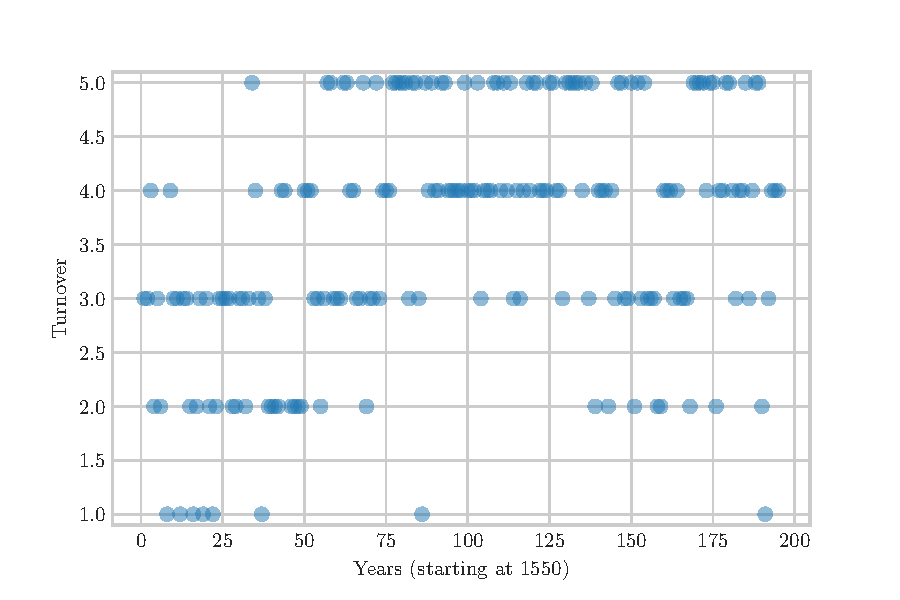
\includegraphics[scale=0.8]{annualturnover5}
	\caption{Absolute turnover of Top5 song topics (1550-1750)}
	\label{fig:annualturnover5}
\end{figure}

\begin{figure}[hbt!]
	\centering
	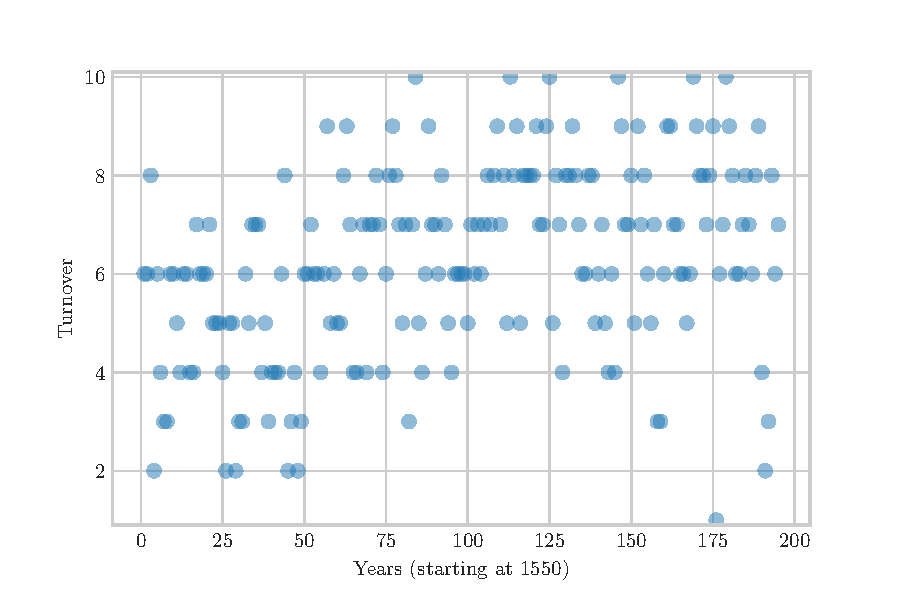
\includegraphics[scale=0.8]{annualturnover10}
	\caption{Absolute turnover of Top10 song topics (1550-1750)}
	\label{fig:annualturnover10}
\end{figure}

The reason why there are no numbers on the x-axis that can be recognized as actual years, is that earlier on, I converted the years to an index, from which five years were excluded of which I had no songs. The shortage of these years slightly distorts the image, but roughly the numbers on the x-axis can be converted to the actual years, by adding 1550 to it. According to Figure~\ref{fig:annualturnover10}, a higher turnover seems to appear from 1600. From 1625 to 1700, a turnover value below 3 does not even appear, which means that during this period, every year at least three new topics appear in the Top10. The same trend can be observed in Figure~\ref{fig:annualturnover5}. Between 1550 and 1600, the number of new topics in the Top5 is located between 1 and 4, but between 1625 and 1700, this number is in general somewhere between 3 and 5. Still, the plots in these figures are not very easy to interpret. Therefore it is helpful to use a smoothing function, which can make the visual intuitions I just made more clear. I use the \enquote{moving average} function, in \texttt{pandas} available through the method \texttt{rolling}. This function takes a couple of datapoints and returns the average of these datapoints. With the argument \texttt{window} I specify the size of the window, i.e. how many previous data points the function should take to calculate the average value. In the following code block I set the window size to 10 and create a plot afterwards:

\begin{lstlisting}
turnover_rw_10 = turnover_topics_10.rolling(10).mean()
plt.rc("text", usetex=True)
plt.rc("font", family="serif")
turnover_rw_10.plot()
\end{lstlisting}

\noindent The same I did for the DataFrame \texttt{turnover\_topics\_5}. Figures~\ref{fig:rolling5} and~\ref{fig:rolling10} show the resulting plots. When looking at Figure~\ref{fig:rolling5} in more detail, I observe a clear increase in turnover regarding the years 1550-1675. Between 1675 and 1720, the line drops, but starts to rise again after 1720. This rise only endures until 1735: by then the line drops again. In Figure~\ref{fig:rolling10}, more or less the same pattern can be observed. This means that starting around 1600, the number of topics that are in the upper part of the ranking in two consecutive years, quickly decreases. In other words: every year, more new topics make their appearance in the Top5 or Top10 of most dominant topics. This confirms the claim that a growing variation in subjects appeared during the seventeenth century.

\begin{figure}[hbt!]
	\centering
	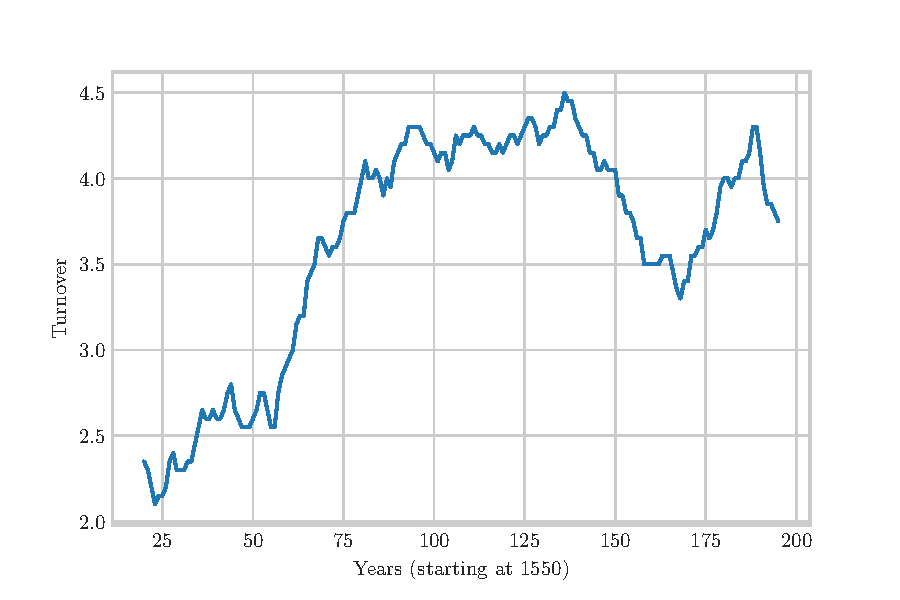
\includegraphics[scale=0.8]{rolling5}
	\caption{Moving average turnover of Top5 song topics (1550-1750, window = 20)}
	\label{fig:rolling5}
\end{figure}

\begin{figure}[hbt!]
	\centering
	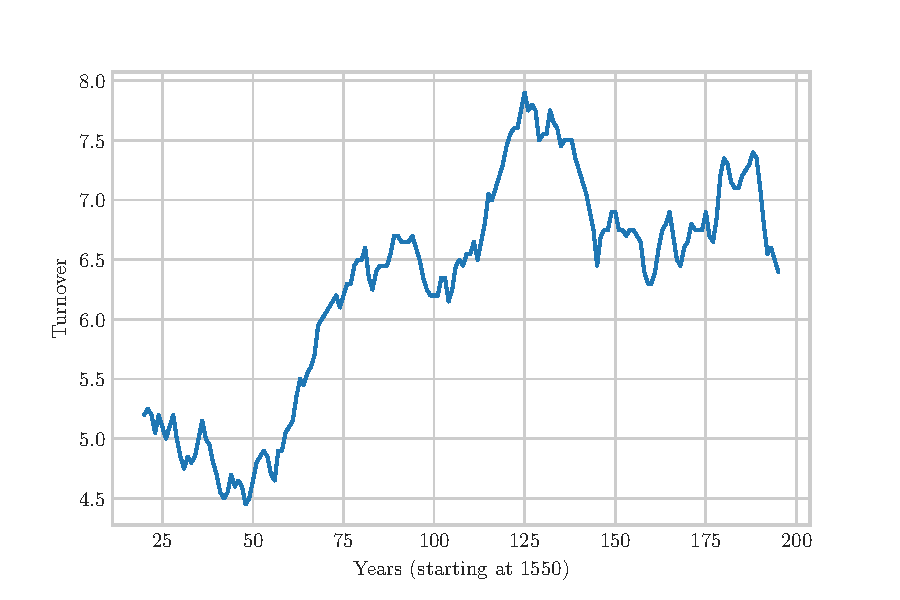
\includegraphics[scale=0.8]{rolling10}
	\caption{Moving average turnover of Top10 song topics (1550-1750, window = 20)}
	\label{fig:rolling10}
\end{figure}

In Chapter 3, I already discussed the different biases that can be at stake in a process of cultural evolution. I mentioned the study of Acerbi and Bentley, who showed a \enquote{concave} turnover profile for the turnover of recent baby names in the United States. The decreasing slope of the curve suggests a preference for relatively uncommon names, which they assign as an anti-conformity bias. The opposite was the case for early boys names, where an increasing slope suggested a preference for common names, in which Acerbi and Bentley recognized a conformity bias. In order to derive a certain bias from a turnover plot, Acerbi and Bentley use a variable top size to calculate the average turnover for each value of the top size. Plotting these two against each other, reveals whether more shifts appear in the bottom of the chart, or in the upper part of the chart. More shifts in the bottom part of the chart results in an increasing slope of the curve and therefore a conformity bias. More shifts in the upper part of the chart results in a decreasing slope of the curve and therefore an anti-conformity bias. In the turnover series that is depicted in Figure~\ref{fig:rolling5}, a fixed top size is used, namely \textit{y} = 5. To create a comparable plot as the ones Acerbi and Bentley plot, I need to calculate the average turnover for every length of the chart. I use the next block of code for that:

\begin{lstlisting}
def slicing(i):
cutoff = df_turnovertop1.iloc[:,0:i]
return cutoff

def turnover(i):
cutoff = slicing(i)
turnco = cutoff.apply(set, axis = 1)
turnovers = {}
for year in range(turnco.index.min() + 1, turnco.index.max() + 1):
name_set, prior_name_set = turnco.loc[year], turnco.loc[year - 1]
turnovers[year] = len(name_set.difference(prior_name_set))
return pd.Series(turnovers)

max_y = 51 
scores = []

for i in range(1, max_y):
avg_turnover = np.mean(turnover(i))
scores.append(avg_turnover)
\end{lstlisting}

In Figure~\ref{fig:turnoverbias51}, the result of the code above is plotted, with \texttt{max\_y} = 51. This means that for every length of the rank (starting with 1), the average turnover is calculated, ending at 50. Looking at the plot, it immediately becomes clear that this curve does not give any insight in possible biases. The reason for that is that in the ranking of song topics, a fixed number of fifty topics fill the charts. The closer the top list size comes to 50, the less topics are excluded, eventually resulting in a turnover of 0: all topics are included in the Top50, so no shifts have taken place. At first it sounds reasonable to create a plot with no negative slope, which means that the top list size should not be larger than 20, but in the end, that would not give extra insight. Since the shape of the curve in Figure~\ref{fig:turnoverbias51} is parabolic, a cutoff would always show a curve with a decreasing slope. According to Acerbi and Bentley, a decreasing slope suggests an anti-conformity bias, but in this case, it is more of a \enquote{parabolic bias}, which has nothing to do with the transmission of traits. Deriving a transmission bias from a turnover plot on early modern song topics will only make sense if the number of different topics is not equal to the maximum top list size.

\begin{figure}[hbt!]
	\centering
	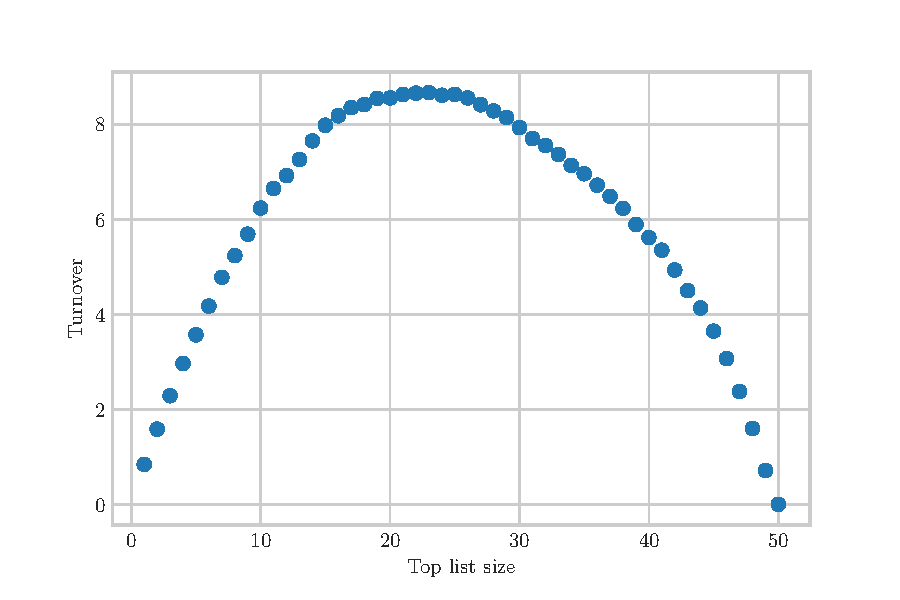
\includegraphics[scale=0.8]{turnoverbias51}
	\caption{Average turnover per top list size}
	\label{fig:turnoverbias51}
\end{figure}


